%%%%%%%%%%%%%%%%%%%%%%%%%%%%%%%%%%%%%%%%%%%%%%%%%%%%%%%%%%%%%%%%%%%%%%%%%%%%%%%%
% Tutorial slides on Python.
%
% Author: Prabhu Ramachandran <prabhu at aero.iitb.ac.in>
% Copyright (c) 2005-2008, Prabhu Ramachandran
%%%%%%%%%%%%%%%%%%%%%%%%%%%%%%%%%%%%%%%%%%%%%%%%%%%%%%%%%%%%%%%%%%%%%%%%%%%%%%%%

\documentclass[14pt,compress]{beamer}
%\documentclass[draft]{beamer}
%\documentclass[compress,handout]{beamer}
%\usepackage{pgfpages} 
%\pgfpagesuselayout{2 on 1}[a4paper,border shrink=5mm]

% Modified from: generic-ornate-15min-45min.de.tex
\mode<presentation>
{
  \usetheme{Warsaw}
  \useoutertheme{split}
  \setbeamercovered{transparent}
}

\usepackage[english]{babel}
\usepackage[latin1]{inputenc}
%\usepackage{times}
\usepackage[T1]{fontenc}

% Taken from Fernando's slides.
\usepackage{ae,aecompl}
\usepackage{mathpazo,courier,euler}
\usepackage[scaled=.95]{helvet}

\definecolor{darkgreen}{rgb}{0,0.5,0}

\usepackage{listings}
\lstset{language=Python,
    basicstyle=\ttfamily\bfseries,
    commentstyle=\color{red}\itshape,
  stringstyle=\color{darkgreen},
  showstringspaces=false,
  keywordstyle=\color{blue}\bfseries}

%%%%%%%%%%%%%%%%%%%%%%%%%%%%%%%%%%%%%%%%%%%%%%%%%%%%%%%%%%%%%%%%%%%%%%
% Macros
\setbeamercolor{emphbar}{bg=blue!20, fg=black}
\newcommand{\emphbar}[1]
{\begin{beamercolorbox}[rounded=true]{emphbar} 
      {#1}
 \end{beamercolorbox}
}
\newcounter{time}
\setcounter{time}{0}
\newcommand{\inctime}[1]{\addtocounter{time}{#1}{\tiny \thetime\ m}}

\newcommand{\typ}[1]{\texttt{#1}}

\newcommand{\kwrd}[1]{ \texttt{\textbf{\color{blue}{#1}}}  }

%%% This is from Fernando's setup.
% \usepackage{color}
% \definecolor{orange}{cmyk}{0,0.4,0.8,0.2}
% % Use and configure listings package for nicely formatted code
% \usepackage{listings}
% \lstset{
%    language=Python,
%    basicstyle=\small\ttfamily,
%    commentstyle=\ttfamily\color{blue},
%    stringstyle=\ttfamily\color{orange},
%    showstringspaces=false,
%    breaklines=true,
%    postbreak = \space\dots
% }


%%%%%%%%%%%%%%%%%%%%%%%%%%%%%%%%%%%%%%%%%%%%%%%%%%%%%%%%%%%%%%%%%%%%%%
% Title page
\title[]{Matrices and Arrays\\ \& \\2D Plotting}

\author[Asokan \& Prabhu] {Asokan Pichai\\Prabhu Ramachandran}

\institute[FOSSEE] {FOSSEE Team}
\date[] {11, October 2009}
%%%%%%%%%%%%%%%%%%%%%%%%%%%%%%%%%%%%%%%%%%%%%%%%%%%%%%%%%%%%%%%%%%%%%%

%\pgfdeclareimage[height=0.75cm]{iitmlogo}{iitmlogo}
%\logo{\pgfuseimage{iitmlogo}}


%% Delete this, if you do not want the table of contents to pop up at
%% the beginning of each subsection:
\AtBeginSubsection[]
{
  \begin{frame}<beamer>
    \frametitle{Outline}
    \tableofcontents[currentsection,currentsubsection]
  \end{frame}
}

\AtBeginSection[]
{
  \begin{frame}<beamer>
    \frametitle{Outline}
    \tableofcontents[currentsection,currentsubsection]
  \end{frame}
}

% If you wish to uncover everything in a step-wise fashion, uncomment
% the following command: 
%\beamerdefaultoverlayspecification{<+->}

%\includeonlyframes{current,current1,current2,current3,current4,current5,current6}

%%%%%%%%%%%%%%%%%%%%%%%%%%%%%%%%%%%%%%%%%%%%%%%%%%%%%%%%%%%%%%%%%%%%%%
% DOCUMENT STARTS
\begin{document}

\begin{frame}
  \maketitle
\end{frame}

\begin{frame}
  \frametitle{Outline}
  \tableofcontents
  % You might wish to add the option [pausesections]
\end{frame}

\section{Matrices and Arrays}

\subsection{Basic \typ{numpy} }

\newcommand{\num}{\texttt{numpy}}

\begin{frame}
  \frametitle{The \num\ module}
  \begin{itemize}
      \item Why?
  \item What:
    \begin{itemize}
    \item An efficient and powerful array type for various common data
      types
    \item Abstracts out the most commonly used standard operations on
      arrays
    \end{itemize}
  \end{itemize}
\end{frame}

\begin{frame}[fragile]
  \frametitle{Examples of \num}
\begin{lstlisting}
# Simple array math example
>>> from numpy import *
>>> a = array([1,2,3,4])
>>> b = array([2,3,4,5])
>>> a*2 + b + 1 # Basic math!
array([5, 8, 11, 14])
# Pi and e are defined.
>>> x = linspace(0.0, 10.0, 1000)
>>> x *= 2*pi/10 # inplace.
# apply functions to array.
>>> y = sin(x)
\end{lstlisting}
\inctime{5}
\end{frame}

\begin{frame}
  \frametitle{Basic concepts}
  \begin{itemize}
  \item fixed size (\typ{arr.size});
  \item Same type (\typ{arr.dtype}) of data
  \item arbitrary dimensionality
  \item \typ{arr.shape}: size in each dimension
  \item \alert{Note:} \typ{len(arr) != arr.size} in general
  \item \alert{Note:} By default array operations are performed
    \alert{elementwise}
  \item Indices, slicing: just like lists 
  \end{itemize}
\end{frame}


\begin{frame}[fragile]
  \frametitle{More examples of \num}
\vspace*{-8pt}
\begin{lstlisting}
>>> x = array([1., 2, 3, 4])
>>> size(x)
4
>>> x.dtype # What is a.dtype?
dtype('float64')
>>> x.shape
(4,)
>>> print rank(x), x.itemsize
1 8
>>> x[0] = 10
>>> print x[0], x[-1]
10.0 4.0
\end{lstlisting}
    
\inctime{10}
\end{frame}

\begin{frame}[fragile]
  \frametitle{Multi-dimensional arrays}
\begin{lstlisting}
>>> a = array([[ 0, 1, 2, 3],
...            [10,11,12,13]])
>>> a.shape # (rows, columns)
(2, 4)
# Accessing and setting values
>>> a[1,3] 
13
>>> a[1,3] = -1
>>> a[1] # The second row
array([10,11,12,-1])

\end{lstlisting}
\end{frame}
\begin{frame}[fragile]
  \frametitle{Array math}
  \begin{itemize}
  \item Basic \alert{elementwise} math (given two arrays \typ{a, b}):
      \typ{+, -, *, /, \%}
  \item Inplace operators: \typ{a += b}, or \typ{add(a, b,
      a)} etc.
  \item Logical operations: \typ{equal (==)}, \typ{not\_equal (!=)},
    \typ{less (<)}, \typ{greater (>)} etc.
  \item Trig and other functions: \typ{sin(x), arcsin(x), sinh(x),
      exp(x), sqrt(x)} etc.
  \item \typ{sum(x, axis=0), product(x, axis=0)} 
  \item \typ{dot(a, bp)}
  \end{itemize}
  \inctime{10}
\end{frame}

\subsection{Array Creation \& Slicing, Striding Arrays}
\begin{frame}[fragile]
  \frametitle{Array creation functions}
  \begin{itemize}
  \item \typ{array(object, dtype=None, \ldots)}
  \item \typ{arange(start, stop=None, step=1 \ldots)}
  \item \typ{linspace(start, stop, num=50, \ldots)}
  \item \typ{ones(shape, dtype=None, \ldots)}
  \item \typ{zeros(shape, dtype=float,\ldots)}
  \item \typ{identity(n)}
  \item \typ{empty(shape, dtype=float,\ldots)}
  \item \typ{ones\_like(x)}, 
  \item \typ{zeros\_like(x)}, \typ{empty\_like(x)}
  \end{itemize}
\end{frame}

\begin{frame}[fragile]
  \frametitle{Slicing arrays}
\begin{lstlisting}
>>> a = array([[1,2,3], [4,5,6], 
               [7,8,9]])
>>> a[0,1:3]
array([2, 3])
>>> a[1:,1:]
array([[5, 6],
       [8, 9]])
>>> a[:,2]
array([3, 6, 9])
\end{lstlisting}
\end{frame}

\begin{frame}[fragile]
  \frametitle{Striding arrays}
\begin{lstlisting}
>>> a[0::2,0::2]
array([[1, 3],
       [7, 9]])
# Slices are references to the 
# same memory!
\end{lstlisting}
\end{frame}

\begin{frame}[fragile]
\frametitle{Random Numbers}
\begin{lstlisting}
>>> np.random.rand(3,2)
array([[ 0.96276665,  0.77174861],
       [ 0.35138557,  0.61462271],
       [ 0.16789255,  0.43848811]])
>>> np.random.randint(1,100)
42
\end{lstlisting}
\inctime{15}
\end{frame}

\begin{frame}[fragile]
  \frametitle{Problem set 1.0}
\inctime{15}
\end{frame}
%%%%%%%%%%%%%%%%%%%%%%%%%%%%%%%%%%%%%%%%%%%%%%%%%%%%%%%%%%%%%%%%%%%%%%

\section{2D Plotting}
\subsection{Getting Started}

\begin{frame}
    {IPython's \typ{pylab} mode}
\begin{itemize}
    \item \typ{pylab}: convenient 2D plotting interface to MPL
    \item Immediate use: \typ{ipython -pylab}
    \item Imports all of pylab for you!
    \item Allows for interactive plotting
\end{itemize}
\end{frame}

\begin{frame}[fragile]
    \frametitle{Basic 2D plotting}

\begin{lstlisting}
>>> x = linspace(0, 2*pi, 1000)
>>> plot(x, sin(x)) 
>>> plot(x, sin(x), 'ro')
>>> xlabel(r'$\chi$', color='g')
# LaTeX markup!
>>> ylabel(r'sin($\chi$)', color='r')
>>> title('Simple figure', fontsize=20)
>>> savefig('/tmp/test.eps')
\end{lstlisting}
\begin{itemize}
  \item Also: PNG, PDF, PS, EPS, SVG, PDF
\end{itemize}
\end{frame}
       
\subsection{Plots - Lines, Labels and Legends}
\begin{frame}[fragile]
  \frametitle{Basic plotting \ldots}
\begin{lstlisting}
# Set properties of objects:
>>> l, = plot(x, sin(x))
# Why "l,"?
>>> setp(l, linewidth=2.0, color='r')
>>> l.set_linewidth(2.0)
>>> draw() # Redraw.
>>> setp(l) # Print properties
>>> clf() # Clear figure.
>>> close() # Close figure.
\end{lstlisting}
\end{frame}

\begin{frame}[fragile]
    \frametitle{Multiple figures}

\begin{lstlisting}
>>> figure(1)
>>> plot(x, sin(x))
>>> figure(2)
>>> plot(x, tanh(x))
>>> figure(1)
>>> title('Easy as 1,2,3')
\end{lstlisting}
    
\end{frame}

\begin{frame}[fragile]
  \frametitle{Legends and Annotation}
\begin{lstlisting}
>>> plot(x, cos(5*x), 'r--', 
         label='cosine')
>>> plot(x, sin(5*x), 'g--', 
         label='sine')
>>> legend() 
# Or use:
>>> legend(['cosine', 'sine'])
# Annotation:
>>> text(1,0, '(1,0)')
\end{lstlisting}
\end{frame}

\begin{frame}[fragile]
    \frametitle{More commands \ldots}
    \begin{lstlisting}
# semilog, loglog 
>>> x = 10.**(-arange(100)*0.1)
>>> semilogx(x, x)
>>> semilogy(x, x)
>>> loglog(x, x)
>>> loglog(x, x*x)
    \end{lstlisting}
\end{frame}

\begin{frame}[fragile]
    \frametitle{More plots \ldots}
    \begin{lstlisting}
>>> clf()
>>> t = arange(0.1, 4, 0.1)
>>> s = exp(-t)
>>> e = 0.1*abs(randn(len(s)))
>>> errorbar(t, s, e)
# Scatter plots
>>> clf()
>>> t = randn(len(e))
>>> scatter(t, e, c=s)
    \end{lstlisting}
\end{frame}

\begin{frame}[fragile]
    \frametitle{Note: \typ{pylab} in Python scripts}
\begin{lstlisting}
import pylab
x = pylab.linspace(0, 20, 1000)
pylab.plot(x, pylab.sin(x))

# Can also use:
from pylab import linspace, sin, plot
\end{lstlisting}
\end{frame}

%%%%%%%%%%%%%%%%%%%%%%%%%%%%%%%%%%%%%%%%%%%%%%%%%%%%%%%%%%%%%%%%%%%%%%
\subsection{Types of Plots}
\begin{frame}[fragile]
  \frametitle{X-Y plot}
  \begin{columns}
    \column{0.5\textwidth}
    \hspace*{-0.5in}
    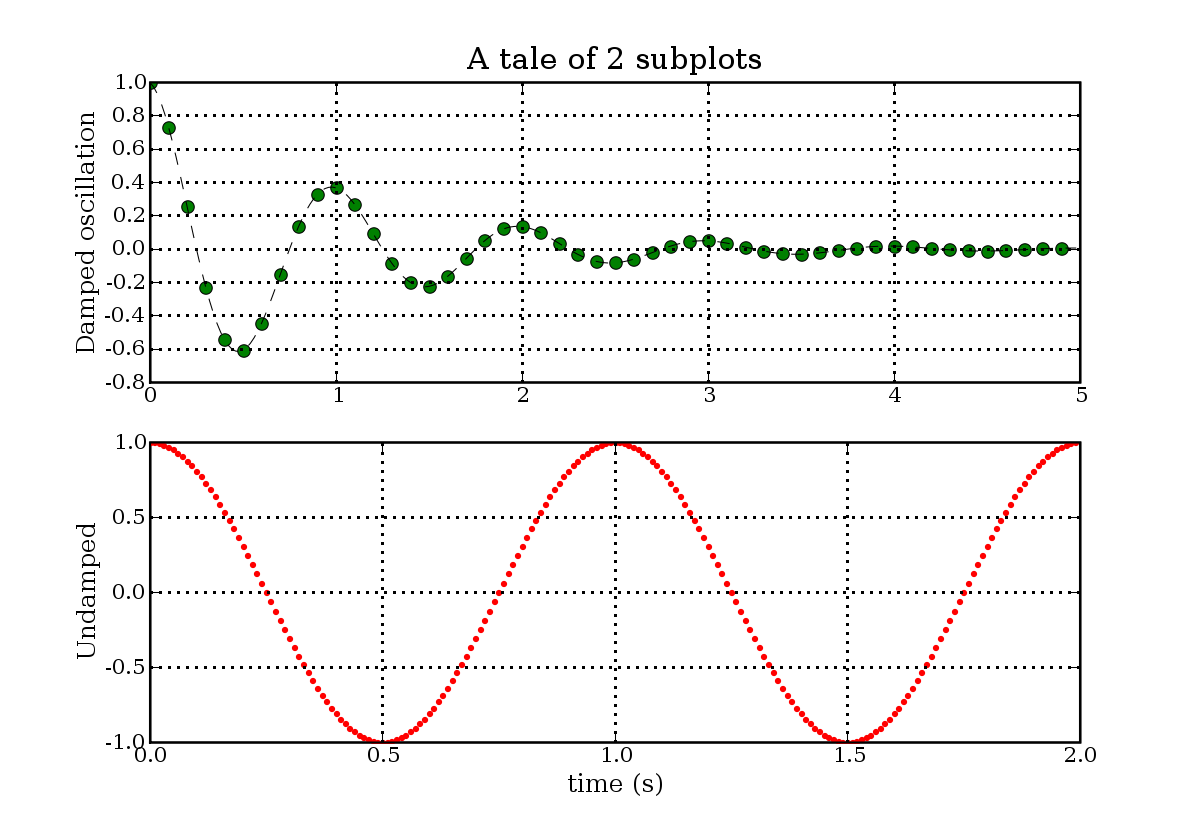
\includegraphics[height=2in, interpolate=true]{data/xyplot}
    \column{0.45\textwidth}
    \begin{block}{Example code}
    \tiny
\begin{lstlisting}
t1 = arange(0.0, 5.0, 0.1)
t2 = arange(0.0, 5.0, 0.02)
t3 = arange(0.0, 2.0, 0.01)
subplot(211)
plot(t1, cos(2*pi*t1)*exp(-t1), 'bo', 
     t2, cos(2*pi*t2)*exp(-t2), 'k')
grid(True)
title('A tale of 2 subplots')
ylabel('Damped')
subplot(212)
plot(t3, cos(2*pi*t3), 'r--')
grid(True)
xlabel('time (s)')
ylabel('Undamped')
\end{lstlisting}
    \end{block}
  \end{columns}
\end{frame}

\begin{frame}[fragile] \frametitle{Semi-log and log-log plots}
  \begin{columns}
    \column{0.5\textwidth}
    \hspace*{-0.5in}
  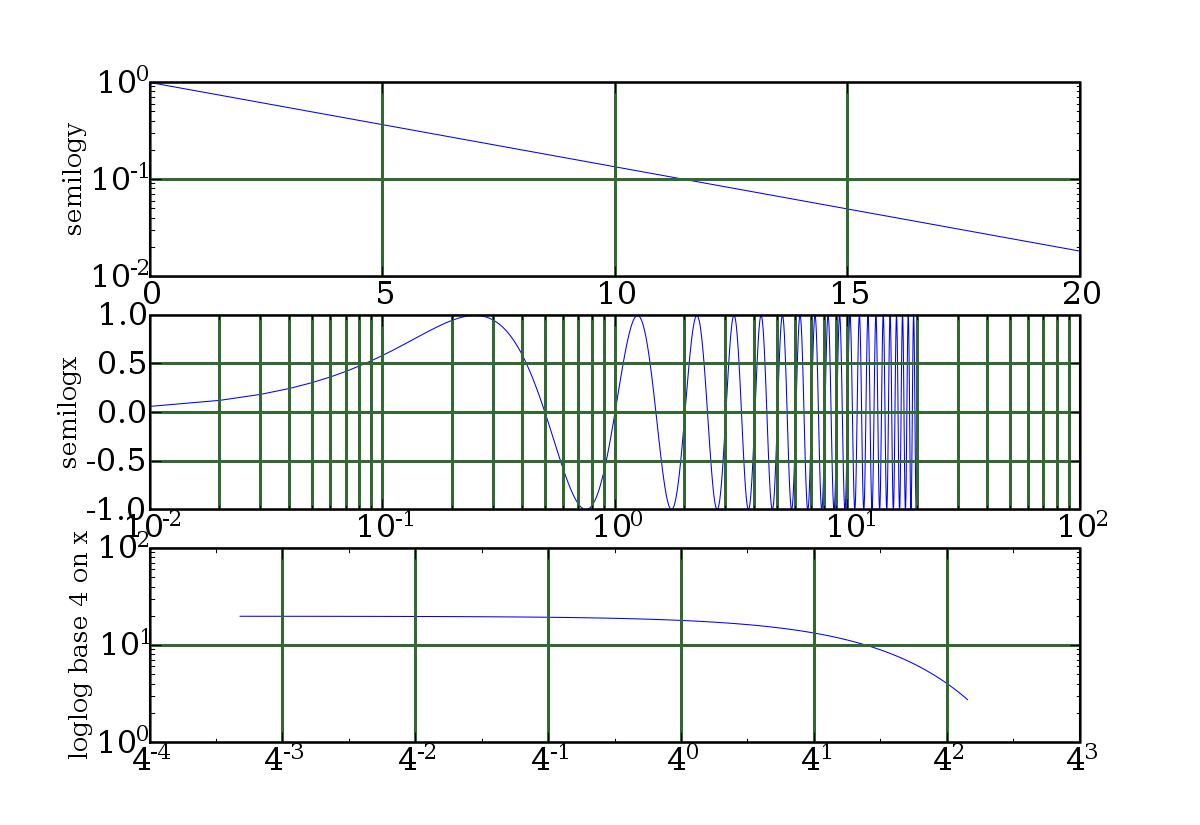
\includegraphics[height=2in, interpolate=true]{data/log}  
    \column{0.45\textwidth}
    \begin{block}{Example code}
    \tiny
\begin{lstlisting}
dt = 0.01
t = arange(dt, 20.0, dt)
subplot(311)
semilogy(t, exp(-t/5.0))
ylabel('semilogy')
grid(True)
subplot(312)
semilogx(t, sin(2*pi*t))
ylabel('semilogx')
grid(True)
# minor grid on too
gca().xaxis.grid(True, which='minor')  
subplot(313)
loglog(t, 20*exp(-t/10.0), basex=4)
grid(True)
ylabel('loglog base 4 on x')
\end{lstlisting}
  \end{block}
\end{columns}
\end{frame}

\begin{frame}[fragile] \frametitle{Errorbar}
  \begin{columns}
    \column{0.5\textwidth}
    \hspace*{-0.5in}
  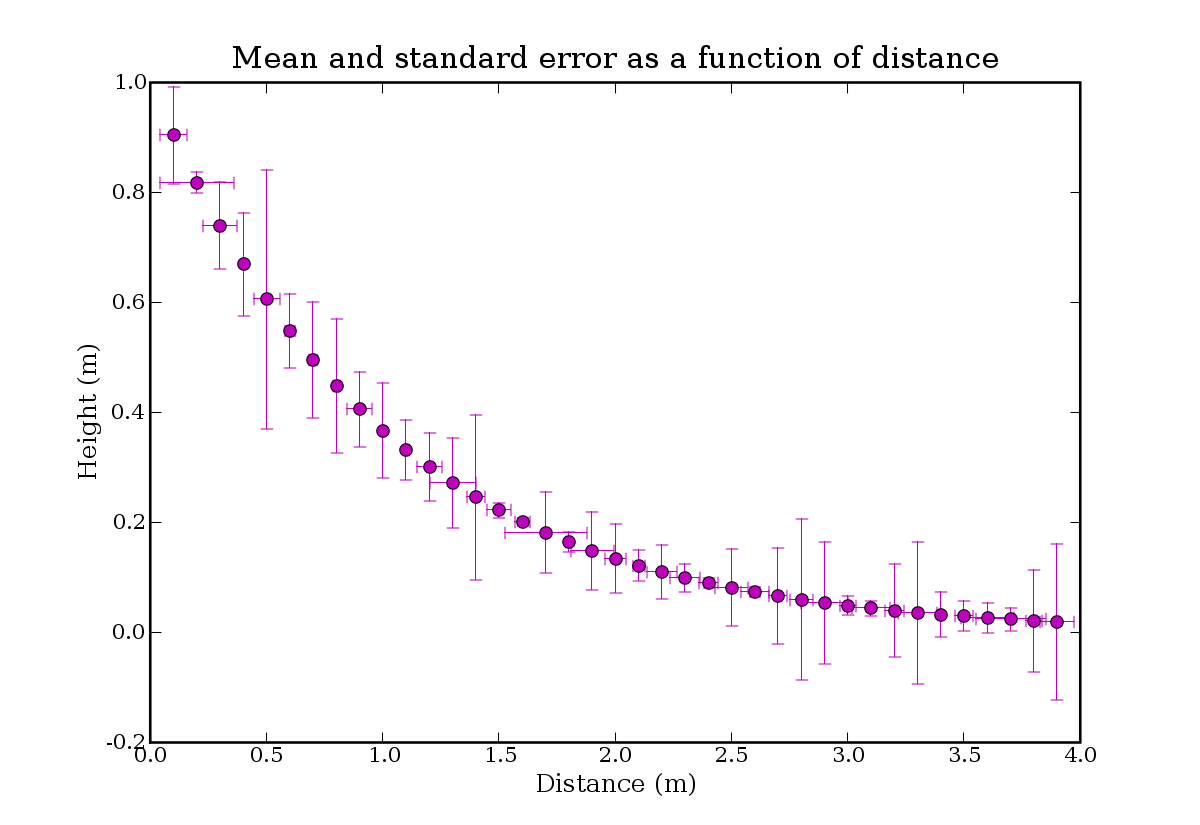
\includegraphics[height=2in, interpolate=true]{data/errorbar}  
    \column{0.45\textwidth}
    \begin{block}{Example code}
    \tiny
\begin{lstlisting}
t = arange(0.1, 4, 0.1)
s = exp(-t)
e = 0.1*abs(randn(len(s)))
f = 0.1*abs(randn(len(s)))
g = 2*e
h = 2*f
errorbar(t, s, [e,g], f, fmt='o')
xlabel('Distance (m)')
ylabel('Height (m)')
title('Mean and standard error '\
      'as a function of distance')
\end{lstlisting}
  \end{block}
\end{columns}
\end{frame}

\begin{frame}[fragile] \frametitle{Histogram}
  \begin{columns}
    \column{0.5\textwidth}
    \hspace*{-0.5in}
  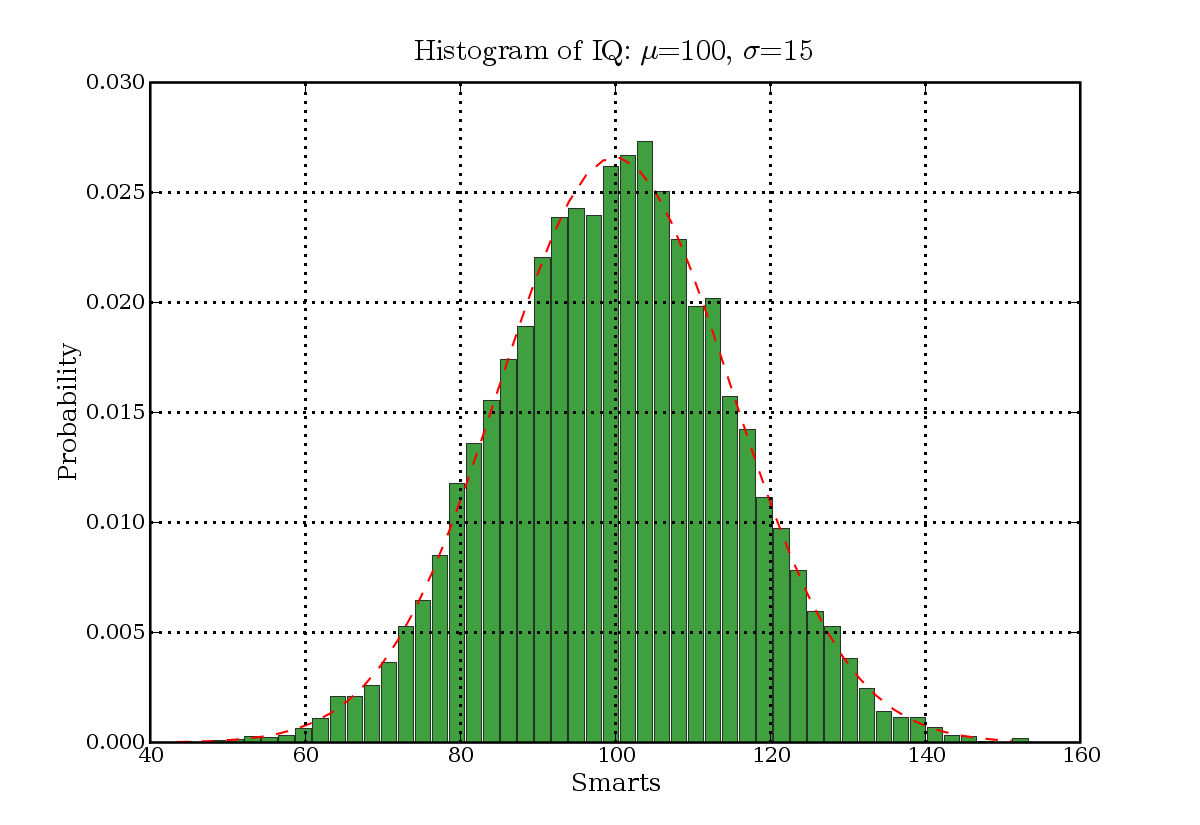
\includegraphics[height=2in, interpolate=true]{data/histogram}  
    \column{0.45\textwidth}
    \begin{block}{Example code}
    \tiny
\begin{lstlisting}
mu, sigma = 100, 15
x = mu + sigma*randn(10000)
# the histogram of the data
n, bins, patches = hist(x, 100, normed=1)
# add a 'best fit' line
y = normpdf( bins, mu, sigma)
l = plot(bins, y, 'r--', linewidth=2)
xlim(40, 160)
xlabel('Smarts')
ylabel('P')
title(r'$\rm{IQ:}\/ \mu=100,\/ \sigma=15$')
\end{lstlisting}
  \end{block}
\end{columns}
\end{frame}

\begin{frame}[fragile] \frametitle{Bar charts}
  \begin{columns}
    \column{0.5\textwidth}
    \hspace*{-0.5in}
  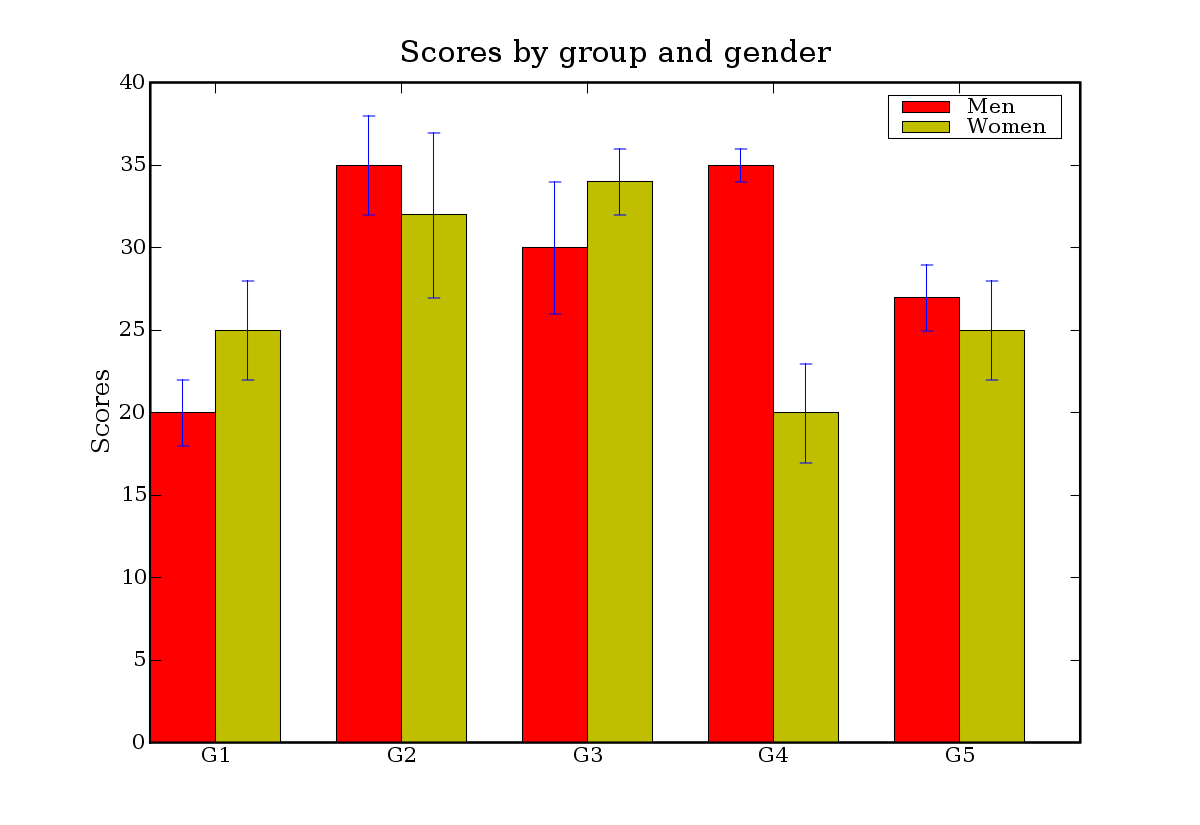
\includegraphics[height=2in, interpolate=true]{data/barchart}  
    \column{0.45\textwidth}
    \begin{block}{Example code}
    \tiny
\begin{lstlisting}
N = 5
menMeans = (20, 35, 30, 35, 27)
menStd =   ( 2,  3,  4,  1,  2)
# the x locations for the groups
ind = arange(N) 
# the width of the bars
width = 0.35       
p1 = bar(ind, menMeans, width, 
         color='r', yerr=menStd)
womenMeans = (25, 32, 34, 20, 25)
womenStd =   ( 3,  5,  2,  3,  3)
p2 = bar(ind+width, womenMeans, width, 
         color='y', yerr=womenStd)
ylabel('Scores')
title('Scores by group and gender')
xticks(ind+width, 
       ('G1', 'G2', 'G3', 'G4', 'G5'))
xlim(-width,len(ind))
yticks(arange(0,41,10))
legend((p1[0], p2[0]), 
       ('Men', 'Women'), shadow=True)
\end{lstlisting}
  \end{block}
\end{columns}
\end{frame}

\begin{frame}[fragile] \frametitle{Pie charts}
  \begin{columns}
    \column{0.5\textwidth}
    \hspace*{-0.4in}
  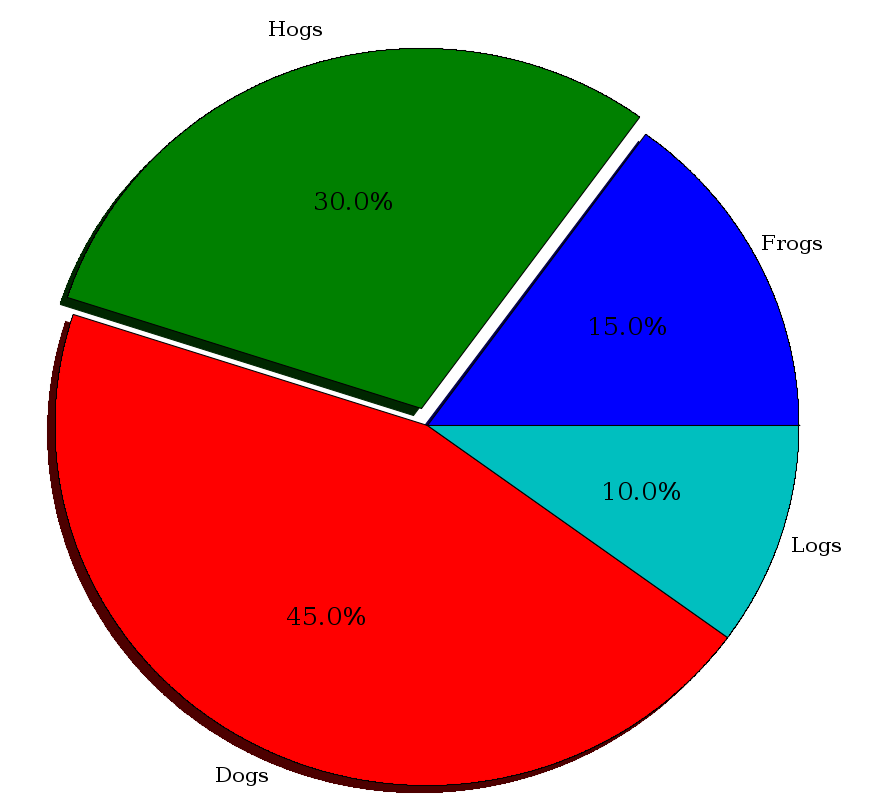
\includegraphics[height=2.0in, interpolate=true]{data/piechart}  
    \column{0.45\textwidth}
    \begin{block}{Example code}
    \tiny
\begin{lstlisting}
# make a square figure and axes
figure(1, figsize=(8,8))
ax = axes([0.1, 0.1, 0.8, 0.8])
labels = 'Frogs', 'Hogs', 'Dogs', 'Logs'
fracs = [15,30,45, 10]
explode=(0, 0.05, 0, 0)
pie(fracs, explode=explode, labels=labels, 
    autopct='%1.1f%%', shadow=True)
title('Raining Hogs and Dogs', 
      bbox={'facecolor':'0.8', 'pad':5})
\end{lstlisting}
  \end{block}
\end{columns}
\end{frame}

\begin{frame}[fragile] \frametitle{Scatter plots}
  \begin{columns}
    \column{0.5\textwidth}
    \hspace*{-0.4in}
  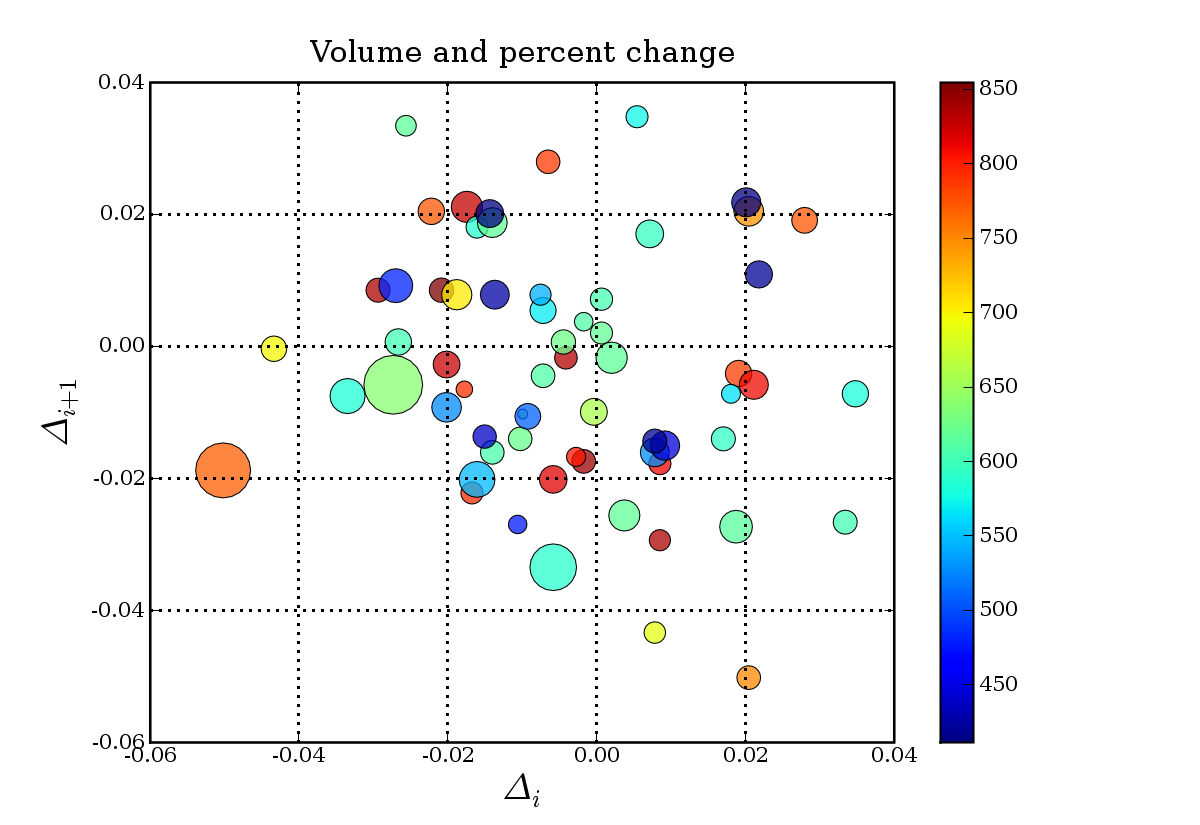
\includegraphics[height=2in, interpolate=true]{data/scatter}  
    \column{0.45\textwidth}
    \begin{block}{Example code}
    \tiny
\begin{lstlisting}
N = 30
x = 0.9*rand(N)
y = 0.9*rand(N)
# 0 to 10 point radiuses
area = pi*(10 * rand(N))**2 
volume = 400 + rand(N)*450
scatter(x,y,s=area, marker='o', c=volume, 
        alpha=0.75)
xlabel(r'$\Delta_i$', size='x-large')
ylabel(r'$\Delta_{i+1}$', size='x-large')
title(r'Volume and percent change')
grid(True)
colorbar()
savefig('scatter')
\end{lstlisting}
  \end{block}
\end{columns}
\end{frame}

\begin{frame}[fragile] \frametitle{Polar}
  \begin{columns}
    \column{0.5\textwidth}
    \hspace*{-0.5in}
  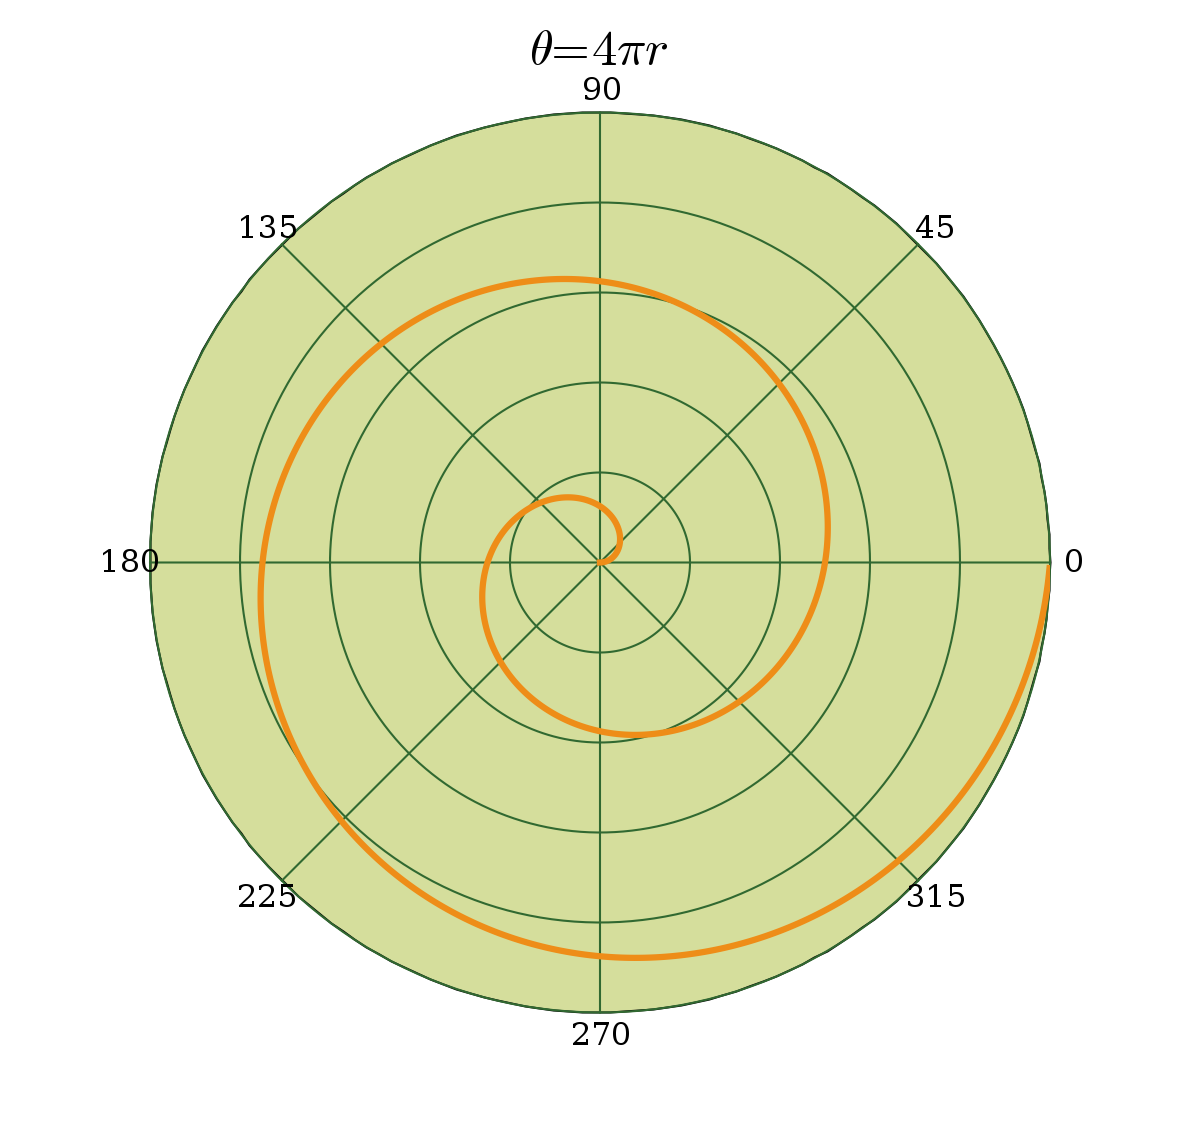
\includegraphics[height=2in, interpolate=true]{data/polar}  
    \column{0.45\textwidth}
    \begin{block}{Example code}
    \tiny
\begin{lstlisting}
figure(figsize=(8,8))
ax = axes([0.1, 0.1, 0.8, 0.8], 
          polar=True, 
          axisbg='#d5de9c')
r = arange(0,1,0.001)
theta = 2*2*pi*r
polar(theta, r, color='#ee8d18', lw=3)
# the radius of the grid labels
setp(ax.thetagridlabels, y=1.075) 
title(r'$\theta=4\pi r$', fontsize=20)
\end{lstlisting}

  \end{block}
\end{columns}
\end{frame}

\begin{frame}[fragile] \frametitle{Contours}
  \begin{columns}
    \column{0.45\textwidth}
    \hspace*{-0.5in}
  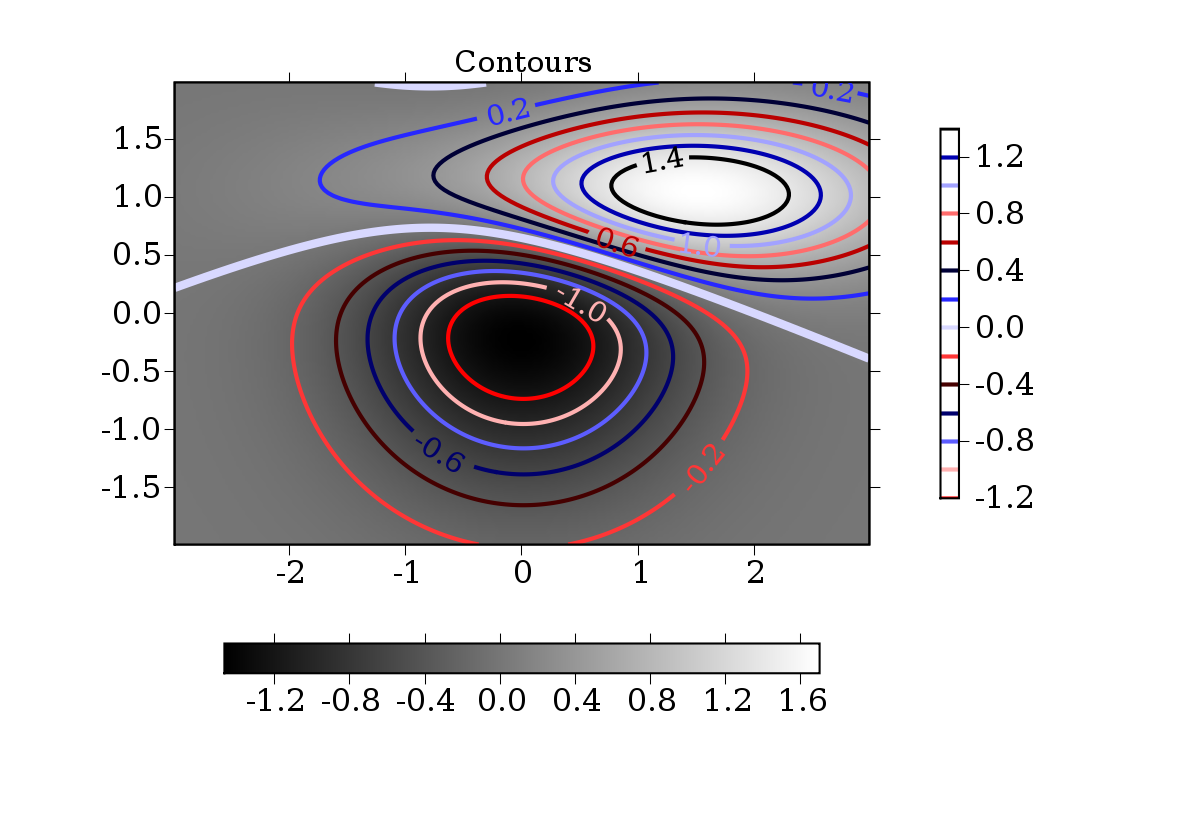
\includegraphics[height=2in, interpolate=true]{data/contour}  
    \column{0.525\textwidth}
    \begin{block}{Example code}
    \tiny
\begin{lstlisting}
x = arange(-3.0, 3.0, 0.025)
y = arange(-2.0, 2.0, 0.025)
X, Y = meshgrid(x, y)
Z1 = bivariate_normal(X, Y, 1.0, 1.0, 0.0, 0.0)
Z2 = bivariate_normal(X, Y, 1.5, 0.5, 1, 1)
# difference of Gaussians
Z = 10.0 * (Z2 - Z1)
im = imshow(Z, interpolation='bilinear', 
            origin='lower',
            cmap=cm.gray, extent=(-3,3,-2,2))
levels = arange(-1.2, 1.6, 0.2)
# label every second level
clabel(CS, levels[1::2],  inline=1,
       fmt='%1.1f', fontsize=14)
CS = contour(Z, levels,
             origin='lower',
             linewidths=2,
             extent=(-3,3,-2,2))
# make a colorbar for the contour lines
CB = colorbar(CS, shrink=0.8, extend='both')
title('Lines with colorbar')
hot(); flag()
\end{lstlisting}
  \end{block}
\end{columns}
\end{frame}

\begin{frame}[fragile] \frametitle{Velocity vectors}
  \begin{columns}
    \column{0.5\textwidth}
    \hspace*{-0.5in}
  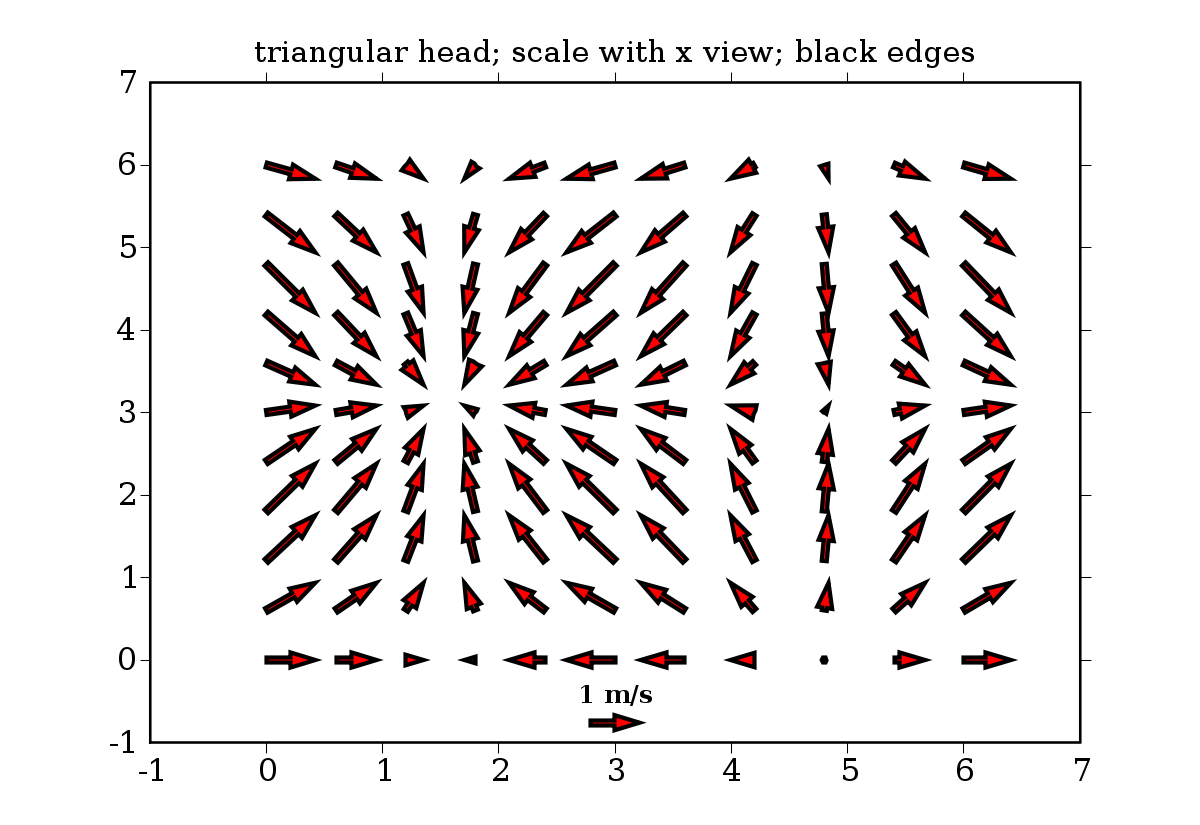
\includegraphics[height=2in, interpolate=true]{data/quiver}  
    \column{0.45\textwidth}
    \begin{block}{Example code}
    \tiny
\begin{lstlisting}
X,Y = meshgrid(arange(0,2*pi,.2),
               arange(0,2*pi,.2) )
U = cos(X)
V = sin(Y)
Q = quiver(X[::3, ::3], Y[::3, ::3], 
           U[::3, ::3], V[::3, ::3],
           color='r', units='x', 
           linewidths=(2,), 
           edgecolors=('k'), 
           headaxislength=5 )
qk = quiverkey(Q, 0.5, 0.03, 1, '1 m/s', 
               fontproperties=
               {'weight': 'bold'})
axis([-1, 7, -1, 7])
title('triangular head; scale '\
      'with x view; black edges')
\end{lstlisting}
  \end{block}
\end{columns}
\end{frame}

\begin{frame}[fragile] \frametitle{Maps}
  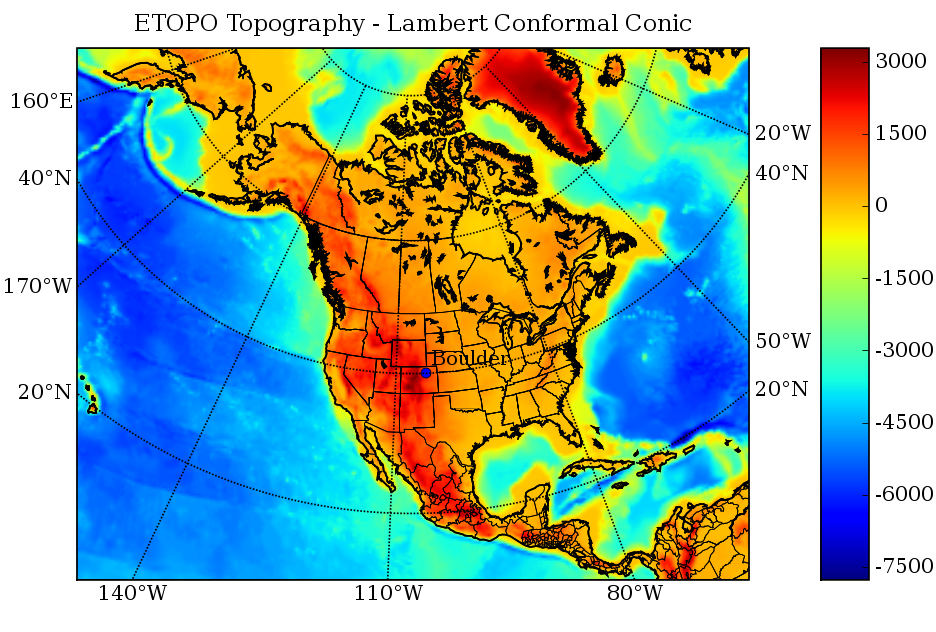
\includegraphics[height=2.5in, interpolate=true]{data/plotmap}  
  \begin{center}
    \tiny
    For details see \url{http://matplotlib.sourceforge.net/screenshots/plotmap.py}
  \end{center}
\end{frame}


\begin{frame}
  \frametitle{More information}
  \begin{itemize}
  \item More information here: \url{http://matplotlib.sf.net}
  \item \url{http://matplotlib.sf.net/tutorial.html}
  \item \url{http://matplotlib.sf.net/screenshots.html}
  \end{itemize}

  \inctime{25}
\end{frame}

\begin{frame}
  \frametitle{Problem set 1.0}
  \begin{enumerate}
      \item Write a function that plots any n-gon given \typ{n}.
      \item Consider the logistic map, $f(x) = kx(1-x)$, plot it for
          $k=2.5, 3.5$ and $4$
\end{enumerate}
\end{frame}

\begin{frame}
  \frametitle{Problem set 1.1}
  \begin{enumerate}
      \item Consider the iteration $x_{n+1} = f(x_n)$ where $f(x) =
          kx(1-x)$.  Plot the successive iterates of this process.
      \item Plot this using a cobweb plot as follows:
          \begin{enumerate}
              \item Start at $(x_0, 0)$
              \item Draw line to $(x_i, f(x_i))$; 
              \item Set $x_{i+1} = f(x_i)$
              \item Draw line to $(x_i, x_i)$
              \item Repeat from 2 for as long as you want 
          \end{enumerate}
    \end{enumerate}
\end{frame}

\begin{frame}
  \frametitle{Problem set 1.2}
  \begin{enumerate}

      \item Plot the Koch snowflake.  Write a function to generate the
          necessary points given the two points constituting a line.
          \pause
          \begin{enumerate}
              \item Split the line into 4 segments.
              \item The first and last segments are trivial.
              \item To rotate the point you can use complex numbers,
                  recall that $z e^{j \theta}$ rotates a point $z$ in 2D
                  by $\theta$.
              \item Do this for all line segments till everything is
                  done.
          \end{enumerate}
      \item Show rate of convergence for a first and second order finite
          difference of sin(x)
\end{enumerate}
\inctime{30}
\end{frame}
\end{document}
